\documentclass[12pt, oneside]{amsart}
\usepackage{amsmath}
\usepackage{lipsum}
\linespread{1.25}
\setlength{\topmargin}{0.in}
\setlength{\oddsidemargin}{0.33in}
\setlength{\textheight}{9.0in}
\setlength{\textwidth}{6.0in}
%-------Packages---------
\usepackage{amssymb,amsfonts}
\usepackage[all,arc]{xy}
\usepackage{enumerate}
\usepackage{mathrsfs}
\usepackage{graphicx}
\usepackage{epstopdf}
\usepackage{listings}
\usepackage{appendix}
\usepackage{listings}
\usepackage{placeins}

%--------Theorem Environments--------
%theoremstyle{plain} --- default
\newtheorem{thm}{Theorem}[section]
\newtheorem{cor}[thm]{Corollary}
\newtheorem{prop}[thm]{Proposition}
\newtheorem{lem}[thm]{Lemma}
\newtheorem{conj}[thm]{Conjecture}
\newtheorem{quest}[thm]{Question}

\theoremstyle{definition}
\newtheorem{defn}[thm]{Definition}
\newtheorem{defns}[thm]{Definitions}
\newtheorem{con}[thm]{Construction}
\newtheorem{exmp}[thm]{Example}
\newtheorem{exmps}[thm]{Examples}
\newtheorem{notn}[thm]{Notation}
\newtheorem{notns}[thm]{Notations}
\newtheorem{addm}[thm]{Addendum}
\newtheorem{exer}[thm]{Exercise}

\theoremstyle{remark}
\newtheorem{rem}[thm]{Remark}
\newtheorem{rems}[thm]{Remarks}
\newtheorem{warn}[thm]{Warning}
\newtheorem{sch}[thm]{Scholium}
\newcommand{\be}{\begin{equation}}
\newcommand{\ee}{\end{equation}}
\makeatletter
\let\c@equation\c@thm
\makeatother
\numberwithin{equation}{section}

\usepackage[style=apa,sortcites=true,sorting=nyt,backend=biber,natbib=true]{biblatex}
%bibliographystyle{unsrtnat}
\addbibresource{Reference/reference.bib}
%%%%%%%%%%%%%%%%%%%%%%%%%%%%%%%%%%%%%%%%%%%%%%%%%%%%%%%%%%%%%%%%%%%%%%%%%%%%%%%%%
% your title/author/date information go here
%--------Meta Data: Fill in your info------


\title{On the MCC-F1 Metric for Binary Classification}

\author{Xuan Li}

\date{September 8, 2024}

\begin{document}

\begin{abstract}
    This report is based on the paper "The MCC-F1 Curve: A Performance Evaluation Technique for Binary Classification" \citep{Cao2020}. There are two sections in this report. The first section provides a comprehensive summary of the paper, discussing the key findings, contributions, limitations and future improvements. The second section includes an extensional study. We firstly investigates further on how severity of imbalance in the datasets affects different metrics. Then we extend to the discussion point on whether there is an optimal classifier across all datasets, in which we conduct simulations and comparisons using machine learning classifiers. 
\end{abstract}
\maketitle
\tableofcontents

%%%%%%%%%%%%%%%%%%%%%%%%%%%%%%%%%%%%%%%%%%%%%%%%%%%%%%%%%%%%%%%%%%%%%%%%%%%%%%%%%section 1

\section{Summary of the Original Paper}

\subsection{Problem Addressed}
The original paper \citep{Cao2020} builds on existing literature regarding evaluation metrics for binary classification problems. Among the commonly used metrics, limitations arise when dealing with imbalanced datasets. The authors discuss methods such as the \textbf{Receiver Operating Characteristic (ROC) curve} and \textbf{Concentrated ROC}, which can be overly optimistic about a classifier's performance when facing negatively skewed datasets, i.e., a high ratio of negative values to true positives \citep{fawcett2006} \citep{swamidass2010}. Additionally, methods like the \textbf{Precision-Recall (PR) curve}
 and \textbf{Precision-Recall-Gain curve} provide limited information when comparing classifier performance on positively skewed datasets or in situations with a high cost for false negatives \citep{swamidass2010} \citep{flach2015}. \\

To address these limitations in evaluating classifier performance on imbalanced datasets, the paper introduces a new evaluation method: the \textbf{MCC-F1 curve} and \textbf{MCC-F1 metric}. This approach combines the normalized \textbf{Matthews Correlation Coefficient (MCC)} with the \textbf{F1 score} \citep{Chicco2020}. The authors argue that the \textbf{MCC-F1} metric is well-suited for evaluating binary classification tasks, regardless of whether the dataset is balanced or imbalanced. Through simulations, the authors show that this new method can outperform commonly used metrics like \textbf{ROC} and \textbf{PR} on imbalanced datasets, overcoming the limitations of existing metrics.


\subsection{MCC-F1 Curve and MCC-F1 Metric}
The newly proposed metric for evaluating binary classifiers, \textbf{MCC-F1}, combines the following two metrics as its major components.
\begin{enumerate}
    \item \textbf{Matthews Correlation Coefficient (MCC)}, provides a comprehensive evaluation of all the elements in the confusion matrix and therefore can handle imbalanced datasets well. $$ MCC=\frac{1}{(TP+FP)(TP+FN)(TN+FP)(TN+FN)}$$
    The value of \textbf{MCC} ranges between $[-1,1]$, where 1 represents a perfect classifier, 0 represents a random classification, and $-1$ represents a completely incorrect classifier. It is important to note that a high \textbf{MCC} value can only be obtained when both true positives and true negatives are high, and both false negatives and false positives are low. 
    \item \textbf{Unit-normalized MCC}, a normalized version of the MCC, is used in both the MCC-F1 curve and the MCC-F1 metric calculation. The formula of \textbf{Unit-normalized MCC} is $$\frac{\textbf{MCC} + 1}{2}$$ The reason for normalization here is to maintain consistency with the \textbf{F1} score, which lies in the range $[0,1]$. 
    \item \textbf{F1 Score}, is the harmonic mean of precision and recall. It is calculated as:
    $$F1=2 \times \frac{Precision \times Recall}{Precision+Recall} $$ The F1 score emphasizes on the balance between precision and recall. It is a commonly used metric when dealing with imbalanced datasets. The value for F1 is between $[0,1]$,
\end{enumerate}

The \textbf{MCC-F1 curve} plots \textbf{unit-normalized MCC} on the Y-axis and \textbf{F1 score} on the X-axis, for different threshold values. This makes it easy to compare how classifiers perform regarding various threshold values. The point $(1,1)$  is the perfect score; it is the best score that a threshold can possibly reach. An example of the \textbf{MCC-F1 curve} plot for a testing classifier with testing dataset and threshold values \{0.1, 0.2, 0.3, 0.4, 0.5, 1.5\} is shown in Figure \ref{figure1}.

\begin{figure}[hbt!]
    \centering
    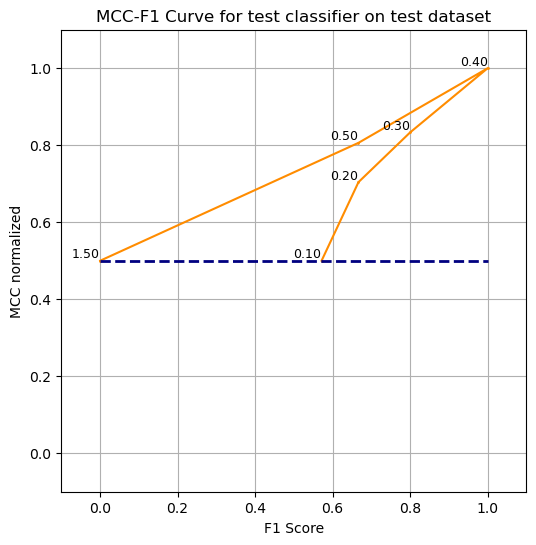
\includegraphics[scale=0.4]{Report/Figure/figure1.jpg}
    \label{figure1}
    \caption{An example of the MCC-F1 curve, with the dashed line representing a random classifier.}
\end{figure}
\FloatBarrier


To give an overall score for a classifier instead of just providing scores at each threshold, the paper introduces the \textbf{MCC-F1 metric}. This is a scale value that summarizes the classifier's overall performance across all threshold values. The process for calculating the MCC-F1 metric as outlined in the paper includes the following key steps:

\textbf{1. Dividing into left and right sides}:
   \begin{itemize}
      \item \textbf{Left side}: threshold values bigger or equal to the best threshold value. 
      \item \textbf{Right side}: threshold values smaller than the best threshold value. 
   \end{itemize}
   This division aims for a balanced evaluation across different threshold values and prediction scores, giving equal weight to both sides. Notice that we've slightly modified the definition from the original paper to make it clearer.
   
\textbf{2. Sub-dividing MCC ranges into sub-ranges}:
   The MCC-F1 curve is split into \textbf{100 sub-ranges} along the MCC axis:
   \[
   \text{subrange size} = \frac{\max(\text{MCC}) - \min(\text{MCC})}{100}
   \]
   This divides the MCC values into equal intervals. For each sub-range, we calculate the mean Euclidean distance from each point in the sub-range to the perfect performance point \((1, 1)\).

\textbf{3. Calculating mean Euclidean distance}:
   For each point \((X_i, Y_i)\) on the MCC-F1 curve, compute the Euclidean distance to the perfect performance point:
   \[
   D_i = \sqrt{(X_i - 1)^2 + (Y_i - 1)^2}
   \]
   where \( X_i \) is the unit-normalized MCC, and \( Y_i \) is the F1 score.

\textbf{4. Averaging over sub-ranges}:
   For each sub-range, calculate the average distance of points within that sub-range \textit{j}:
   \[
   \bar{D_j} = \frac{\sum_{i \in \text{sub-range}} D_i}{n_j}
   \]
   where \( n_j \) is the number of points in the sub-range \textit{j}.

\textbf{5. Grand average distance}:
   The grand average distance \( D^* \) is calculated as the average of all sub-range mean distances across both left and right sides:
   \[
   D^* = \frac{\sum_{(s, j)} \bar{D_j}}{|P|}
   \]
   where \( P \) is the set of sub-ranges with non-zero points.

\textbf{6. Final MCC-F1 metric}:
   The final MCC-F1 metric is calculated as:
   \[
   \text{MCC-F1 metric} = 1 - \frac{D^*}{\sqrt{2}}
   \]
   This value ranges from 0 to 1, with a value of 1 indicating perfect performance.
\\

This approach provides a balanced evaluation of classifier performance across different prediction thresholds while avoiding bias from uneven distribution of points. An example of the right-left sides and sub-range division plot is shown in Figure \ref{figure2}. 
\begin{figure}[hbt!]
    \centering
    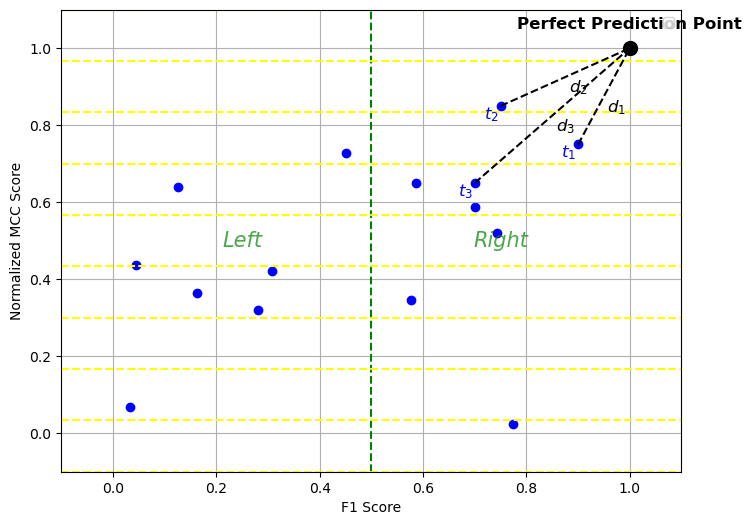
\includegraphics[scale=0.3]{Report/Figure/figure2.jpg}
    \label{figure2}
    \caption{The green dashed line divides the points into left and right sides, and the yellow dashed lines divides the points into sub-ranges. }
\end{figure}
\FloatBarrier





\subsection{Comparison to Other Metrics}
The paper compares MCC-F1 with ROC and PR through simulations under different datasets. The experiment includes 2 classifiers and 3 datasets.  The 3 simulated datasets only differ in their ground truth values of 0 and 1. Since this is a binary classification setup, 0 represents the negative class and 1 represents the positive class. They are the only possible outcomes. Dataset X is skewed toward the negative class, with 1,000 positives and 10,000 negatives. Dataset Y is skewed toward the positive class, with 10,000 positives and 1,000 negatives. Dataset Z is perfectly balanced, containing 10,000 positives and 10,000 negatives. \\

The authors simulate prediction scores for two classifiers using different Beta distributions. For \textbf{classifier A}, they use a Beta(12, 2) distribution for the first 30\% of positive cases and Beta(3, 4) for the remaining positives. This approach models a classifier with high recall at higher thresholds and lower recall at lower thresholds. For negative cases, they sample scores from Beta(2, 3). For \textbf{classifier B}, the scores for positive cases are all sampled from Beta(4, 3), and the negative cases are sampled from the Beta(2, 3). \\
\\
\underline{\textbf{Negatively Imbalanced Dataset:}}
For this dataset,  \textbf{classifier B} appears to perform better than \textbf{classifier A} in the ROC analysis (with an AUROC value of 0.73 for \textbf{classifier B} and 0.69 for \textbf{classifier A}). However, in the PR analysis, \textbf{classifier A} has a clear advantage when recall is below 0.4 but when recall exceeds 0.4, the difference between them is small. The overall AUPR value is 0.3 for \textbf{classifier A} and 0.2 for \textbf{classifier B}. In the MCC-F1 analysis, \textbf{classifier A} outperforms \textbf{classifier B}, with a better MCC-F1 curve and a higher score (0.35 for \textbf{classifier A} and 0.34 for \textbf{classifier B}). This result shows that \textbf{classifier B} does not perform as well as the ROC analysis suggests. ROC curves can be misleading in cases with a big imbalance between negative and positive classes.
\\
\underline{\textbf{Positively Imbalanced Dataset:}}
For this dataset, \textbf{classifier A} and  \textbf{classifier B} appear to perform similarly (almost identical) in the PR analysis (with the same AUPR value of 0.96 for both \textbf{classifier A} and \textbf{classifier B}). However, in the ROC analysis, \textbf{classifier B} has a clear advantage over \textbf{classifier A} in the plot. And the overall AUROC value is 0.69 for \textbf{classifier A} and 0.73 for \textbf{classifier B}. In the MCC-F1 analysis, both classifiers appear to perform closely when F1 $<$ 0.62 but when F1 exceeds 0.62, \textbf{classifier B} outperforms \textbf{classifier A} clearly.  The overall MCC-F1 value is 0.49 for \textbf{classifier A} and 0.59 for \textbf{classifier B}. This result shows that PR is much less informative than AUC and MCC-F1 under positively imbalanced datasets. \\
\\
\underline{\textbf{Balanced Dataset:}}
For this dataset, \textbf{classifier A} and \textbf{classifier B} appear to perform similarly in all three analysis (ROC, PR and MCC-F1). The plots show that the ROC, PR and MCC-F1 curves for two classifiers cross each other at some point. Both classifiers have the same AUPR value of 0.71. The AUROC value is 0.69 for \textbf{classifier A} and 0.73 for \textbf{classifier B}. The MCC-F1 value is 0.46 for \textbf{classifier A} and 0.53 for \textbf{classifier B}. This result shows that MCC-F1 metric has a bigger difference between the two classifiers.  Therefore the MCC-F1 metric makes it more clear to select the best classifier than ROC and PR analysis. \\
\\
In summary, MCC-F1 outperforms ROC and PR in many of the situations including the three cases discussed above. The \textbf{MCC-F1} analysis provides a more complete evaluation by considering all elements of the confusion matrix, making it particularly useful for imbalanced datasets as well as balanced ones. And it provides a straightforward way to select the best thresholds value.

\subsection{Highlights, Limitations and Future Improvements}
Imbalanced datasets are common in the real-world, especially in areas like medicine, genomics, and fraud detection. In these situations, the MCC-F1 curve provides a more accurate and fair way to assess classifier performance. This is a key contribution of the paper. Additionally, MCC-F1 curve presents a straightforward view to identify the best threshold value. Identifying the best threshold for a classifier is critical in real-world applications, especially when the cost of false positives and false negatives is unequal. The MCC-F1 metric also simplifies comparisons between classifiers by offering a single value, the MCC-F1 metric, which can summarize overall performance. While the MCC-F1 curve and metric provide clear advantages, there are some limitations. \\

One limitation of the MCC-F1 analysis in the original paper is the \textbf{lack of theoretical justification}. This includes elaboration on why combining MCC and F1 works as an effective metric. The paper introduces this combination and claims it works based on the nature of MCC and F1 metrics, but does not provide enough detail to explain why this metric is valid or superior, and how it is better than just using MCC or F1 metric alone. Additionally, the MCC-F1 metric formula \textbf{leaves some ambiguity}. For instance, the division of the left and right side in metric calculation is unclear. The original paper states that the division is based on the best prediction score (detail in page 7 of \citep{Cao2020}), but achieving a score better than the best score is not possible. This would result in the left side having only a single point, which is the threshold with the best prediction score. Furthermore, in extreme cases where one side is empty, the paper does not specify how to handle that. Should we simply assign zero for the missing side and divide to get the average, or rely solely on the available side's value? The paper also lacks guidance on the optimal number of sub-ranges division for balancing accuracy and computational cost, making it unclear why dividing into 100 sub-ranges adds value. Dividing into too many sub-ranges, when fewer threshold values exist, seems excessive and unnecessary. These gaps in the explanation create uncertainty on how to apply the metric in practice.\\

One limitation of the MCC-F1 analysis is the \textbf{complexity of interpretation}. While it combines two important metrics, the complexity of the structure also increases. In fact, MCC itself is often viewed as harder to interpret than more straightforward metrics like AUC and PR. For practitioners who preferred interpretable methods, the complexity in the MCC-F1 metric potentially requires additional explanation and interpretation of its outcome. Another challenge is its \textbf{scalability to extend to multi-class problems}. The paper focuses solely on binary classification setting. Adapting the MCC-F1 curve to multi-class classification setting would require modifications for the re-structuring of the metric. Since this metric requires more computation than just comparing existing evaluations, it also adds complexity when extending to a broader range of use cases. Lastly, the paper's findings are heavily based on \textbf{simulation data}. How well the MCC-F1 curve performs in real-world datasets remains unknown. We propose several directions for future improvements and further analysis.
\begin{enumerate}
    \item We can explore different left-right division methods, such as using the mean or median F1 score. Since the current method relies on MCC for sub-range division, similar approaches using F1 score could be tested. In a quick simulation, we found that different division methods, like median and mean F1 scores, resulted in more balanced outcomes depending on the specific dataset and classifier. How to choose the most appropriate division when calculating the MCC-F1 metric under different cases can be investigated. The plots of different division methods in our simulation are shown in Figure \ref{division}. 
    \begin{figure}[hbt!]
        \centering
        \setlength{\unitlength}{\textwidth} 
        \begin{picture}(1,0.5)%in case your image is twice as wide as it is high.
            \put(-0.12,0){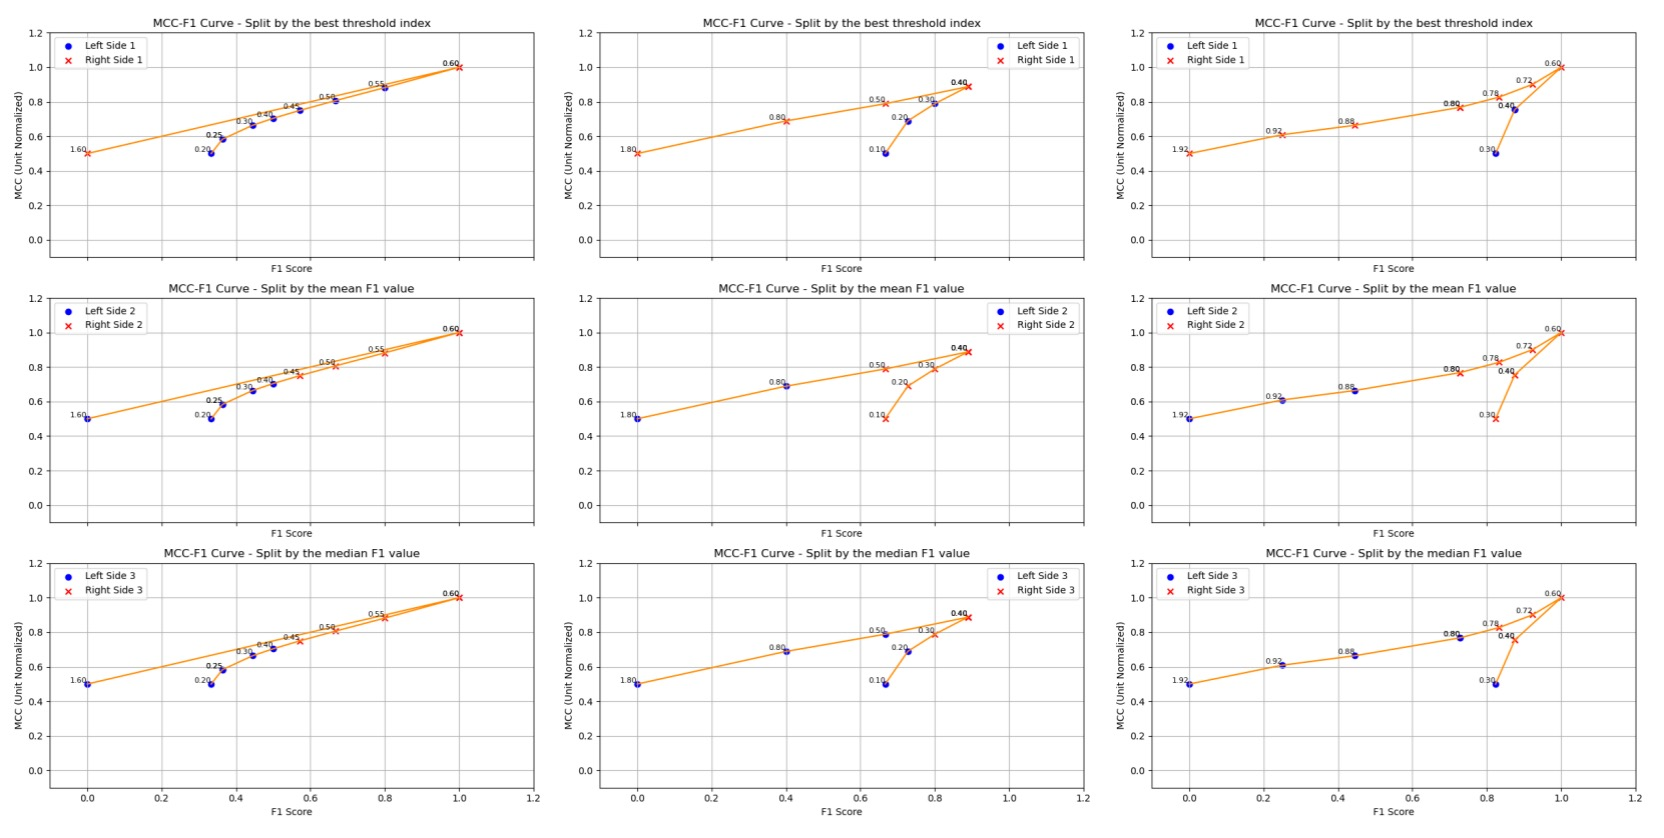
\includegraphics[width=1.25\unitlength]{Report/Figure/division.jpg}}
        \end{picture}
        \caption{Different divisions for (1) Negatively skewed dataset, (2) balanced dataset, and (3) positively skewed dataset}
        \label{division}
    \end{figure}
    \FloatBarrier

    \item We can extend the analysis to multi-class classification with some adjustments to the formula. Alternative approaches to structure the multi-class analysis should be considered. For instance, the confusion matrix can be an $N \times N$ matrix. Each row of the matrix represents the actual class (true labels), and each column represents the predicted class. Alternatively, we can simplify the multi-class confusion matrix by just treating it as a binary classification problem (i.e., treating each prediction as either correct or incorrect, without distinguishing between specific classes). 
    \item \textbf{Proposed by Prof. Keegan Korthauer}: A deeper analysis is needed to explore whether the severity of imbalance affects certain metrics more than others. This can be examined both analytically and through simulations.
    \item \textbf{Proposed by Prof. Keegan Korthauer}: A key discussion point is whether the balance between positive and negative classes should influence the choice of optimal classifier. Is it possible for one classifier to universally outperform others?
    \item Finally, we propose comparing the performance of the MCC-F1 metric not only against ROC and PR analyses but also against other methods like MCC, F1, Balanced Accuracy, G-Mean (Geometric Mean), Fowlkes-Mallows Index (FMI), and so on. One can apply and compare these methods on real-world datasets to better understand their effectiveness in practical scenarios.
\end{enumerate}
%%%%%%%%%%%%%%%%%%%%%%%%%%%%%%%%%%%%%%%%%%%%%%%%%%%%%%%%%%%%%%%%%%%%%%%%%%%%%%%%%
\section{Extensional analysis}
In this section, we explore the topics on items \textbf{3} and \textbf{4} from the list of proposed future improvements. We address these two discussion points in separate subsections. For each, we set up simulations in Python for our investigation.

\subsection{Severity of imbalance in different metrics}
We explore how the severity of imbalance affects different metrics. Specifically, we focus on a limited set of metrics: \textbf{ROC} (\textbf{AUC ROC} in the following figures stands for \textbf{Area Under Curve for ROC}), \textbf{PR} (\textbf{AUC PR} stands for \textbf{Area Under Curve for PR}), and \textbf{MCC-F1}. In the first simulation experiment, we generate datasets ranging from negatively skewed to positively skewed. Our approach adjusts the ratio between the number of positives and negatives, while keeping the total number of data points fixed at 10,000 for each dataset. The ratio is adjusted from 1:49 to 49:1 over 13 datasets. This means that in the first dataset, we have 200 positives and 9,800 negatives. We adjust the ratio gradually. For the 7th dataset, we have a perfectly balanced dataset with 5,000 positives and 5,000 negatives, and for the 13th dataset, we have 9,800 positives and 200 negatives. Results are presented in Figure \ref{simulation1}. We applied two classifiers to the datasets, which are generated using the same processes as in the original paper, employing beta distributions. \\


Our simulation shows that as the ratio between positives and negatives changes, both the \textbf{MCC-F1 metric} and \textbf{AUPR} change accordingly. There is a positive relationship between the ratio and these metrics: as the number of positives increases and the number of negatives decreases, the \textbf{MCC-F1 metric} and \textbf{AUPR} improve. In contrast, the \textbf{AUROC} remains relatively stationary across different ratios for both classifiers.\\

When comparing the two classifiers, \textbf{AUROC} consistently shows that \textbf{classifier B} outperforms \textbf{classifier A}. \textbf{MCC-F1} follows this trend, except for the first several extremely negatively skewed datasets, where classifier A performs better. \textbf{AUPR}, however, initially favors \textbf{classifier A} but gradually overlaps with \textbf{classifier B} as the dataset becomes more positively skewed. This aligns with the authors' observation that \textbf{PR} curve can be less informative for classifier comparison on positively skewed datasets. In our case, the overlap occurs just after the balanced dataset.\\

Given how we build the classifiers, it makes sense why \textbf{classifier B} performs better overall. \textbf{Classifier A} generates 70\% of positives using a beta(3,4) distribution, while \textbf{classifier B} generates 100\% of positives using beta(4,3). As the dataset becomes more dominated by positives, \textbf{classifier B}'s advantage on identify positives leads to an overall better performance.\\

\begin{figure}
    \centering
    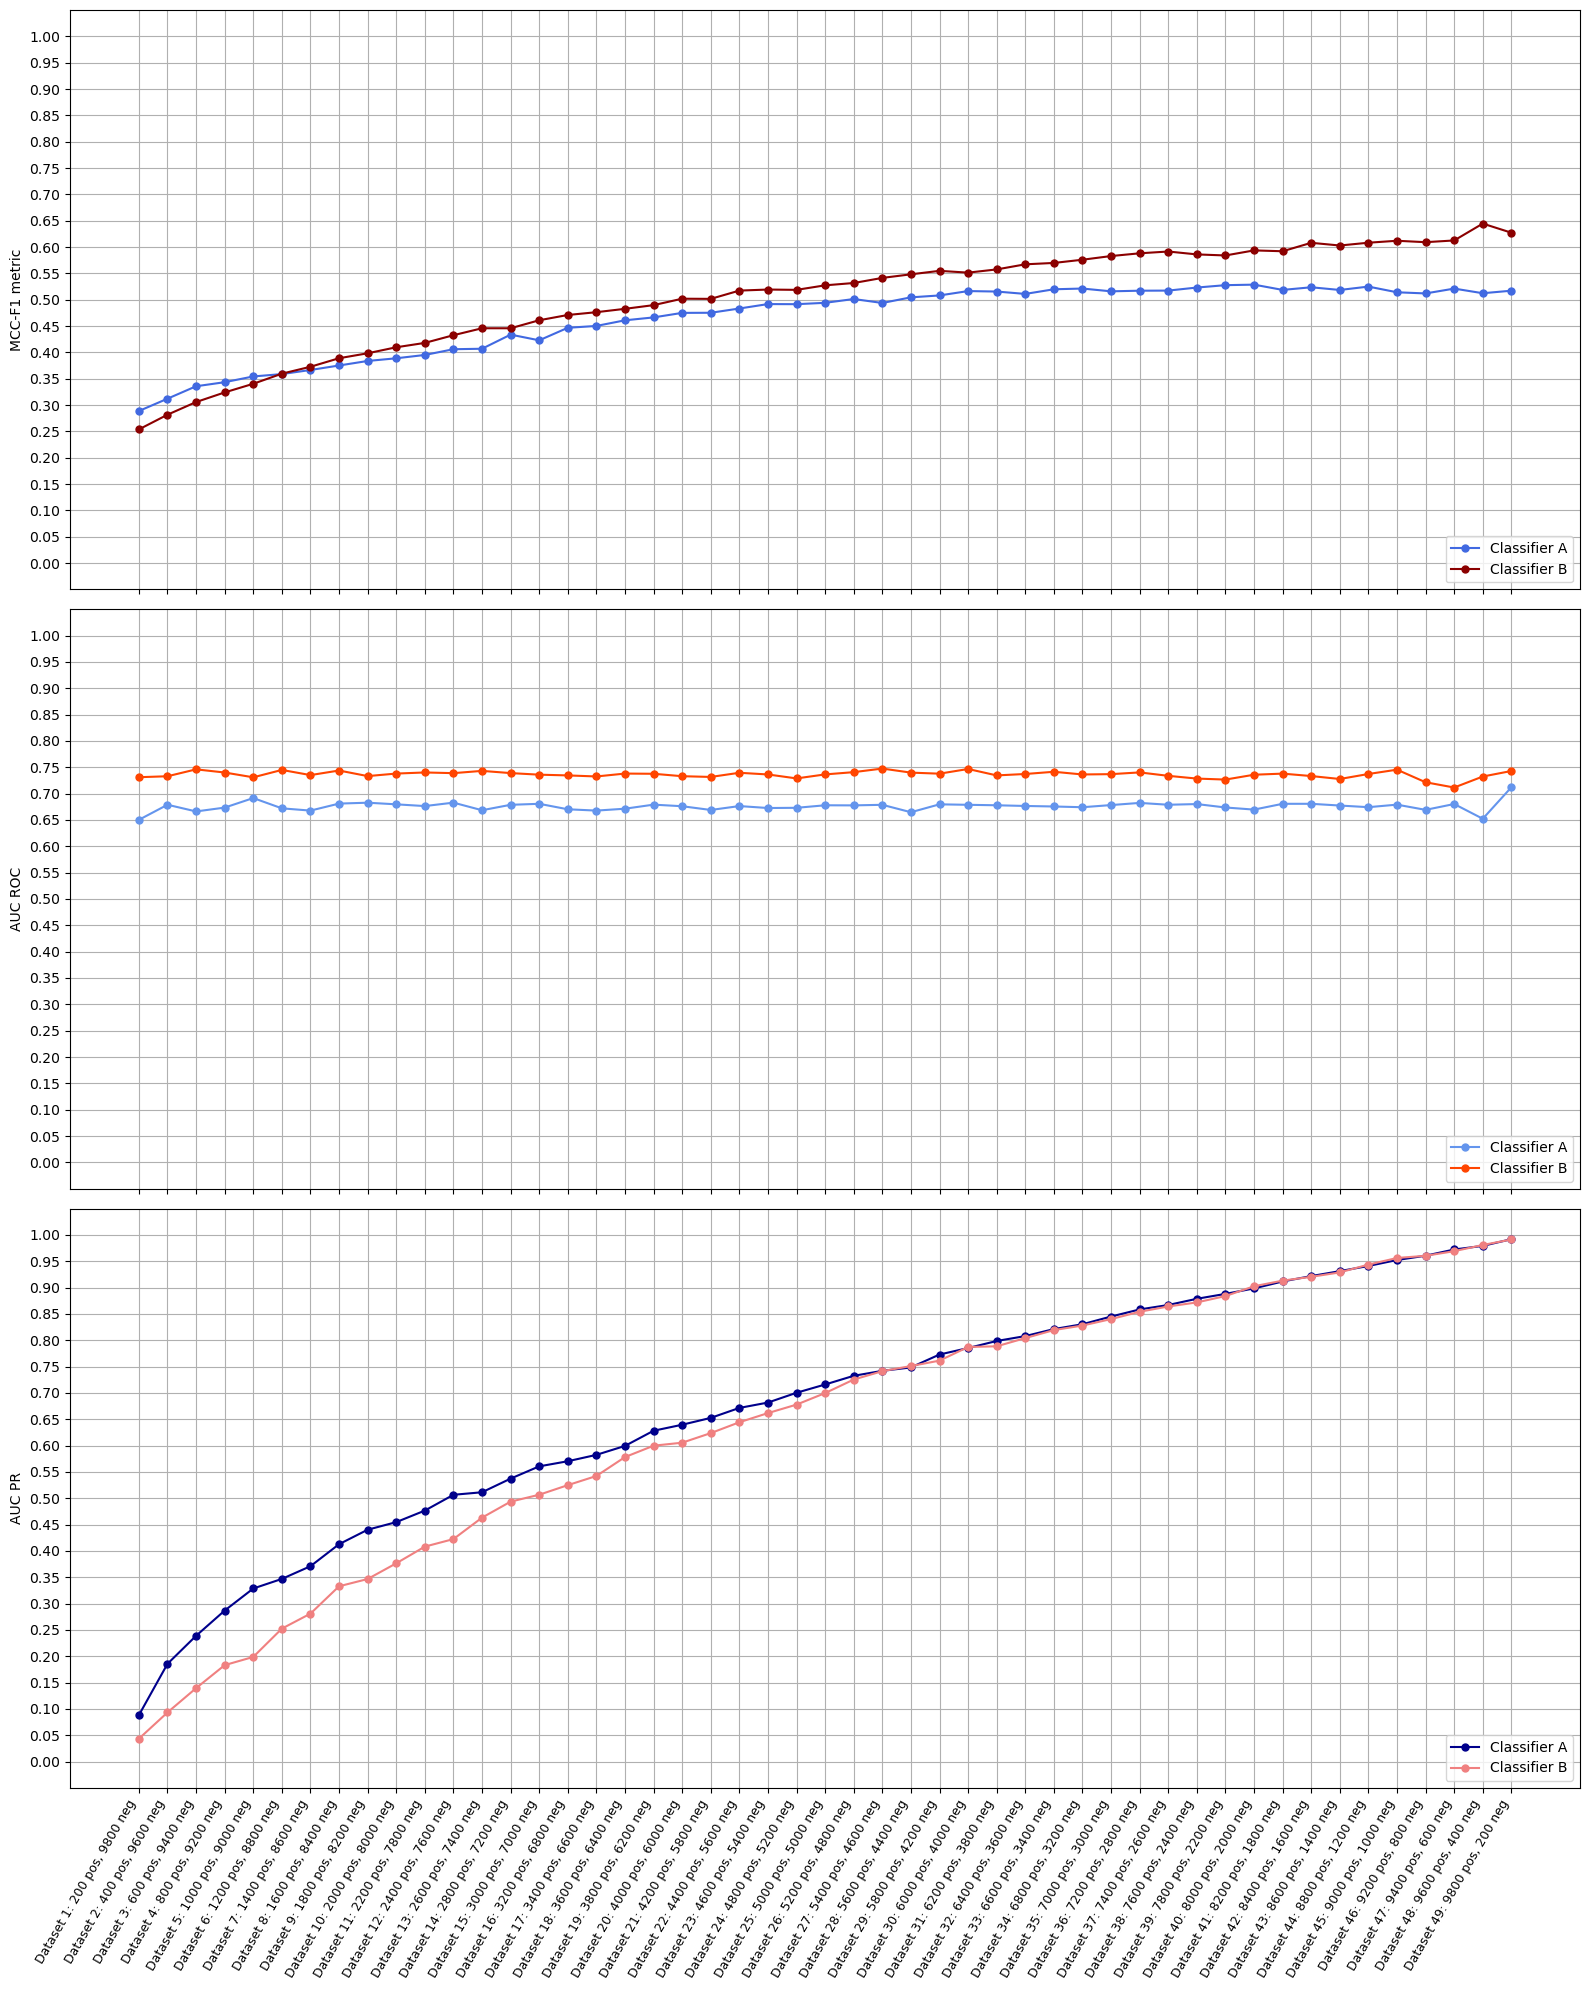
\includegraphics[scale=0.28]{Report/Figure/simulation1.jpg}
    \caption{Metric values with respect to variations in datasets of different positives: negative ratios for (1) MCC-F1 metric, (2) the area under curve for ROC, and (3) the area under curve for PR}
    \label{simulation1}
\end{figure}


In the second simulation experiment, we perform a relative sensitivity analysis for \textbf{MCC-F1 metric}, \textbf{AUROC}, and \textbf{AUPR}. We plot the percentage changes in classifier performance relative to the perfectly balanced dataset. We use the following formula: $$metricPctChange = \frac{metricScore_i - metricScore_b}{metricScore_b}$$ where $metricScore_i$ is the score of the metric for dataset $i$, and $metricScore_b$ is the score of the metric for the perfectly balanced dataset. The percentage change values are rounded to two decimal places. Results are plotted in Figure \ref{simulation2}. \\

As shown in the plots, the percentage change for \textbf{AUROC} remains quite stable for both classifiers. This indicates that, regardless of the class imbalance in the dataset, the \textbf{AUROC} does not vary much for the same classifier. In contrast, the percentage changes for both \textbf{AUPR} and the \textbf{MCC-F1 metric} are much more pronounced. These metrics are sensitive to class imbalance. However, the percentage changes for \textbf{AUPR} are very similar across classifiers, while the percentage changes for the \textbf{MCC-F1 metric} show more noticeable differences. Results are shown in figure \ref{simulation2}.

\begin{figure}
    \centering
    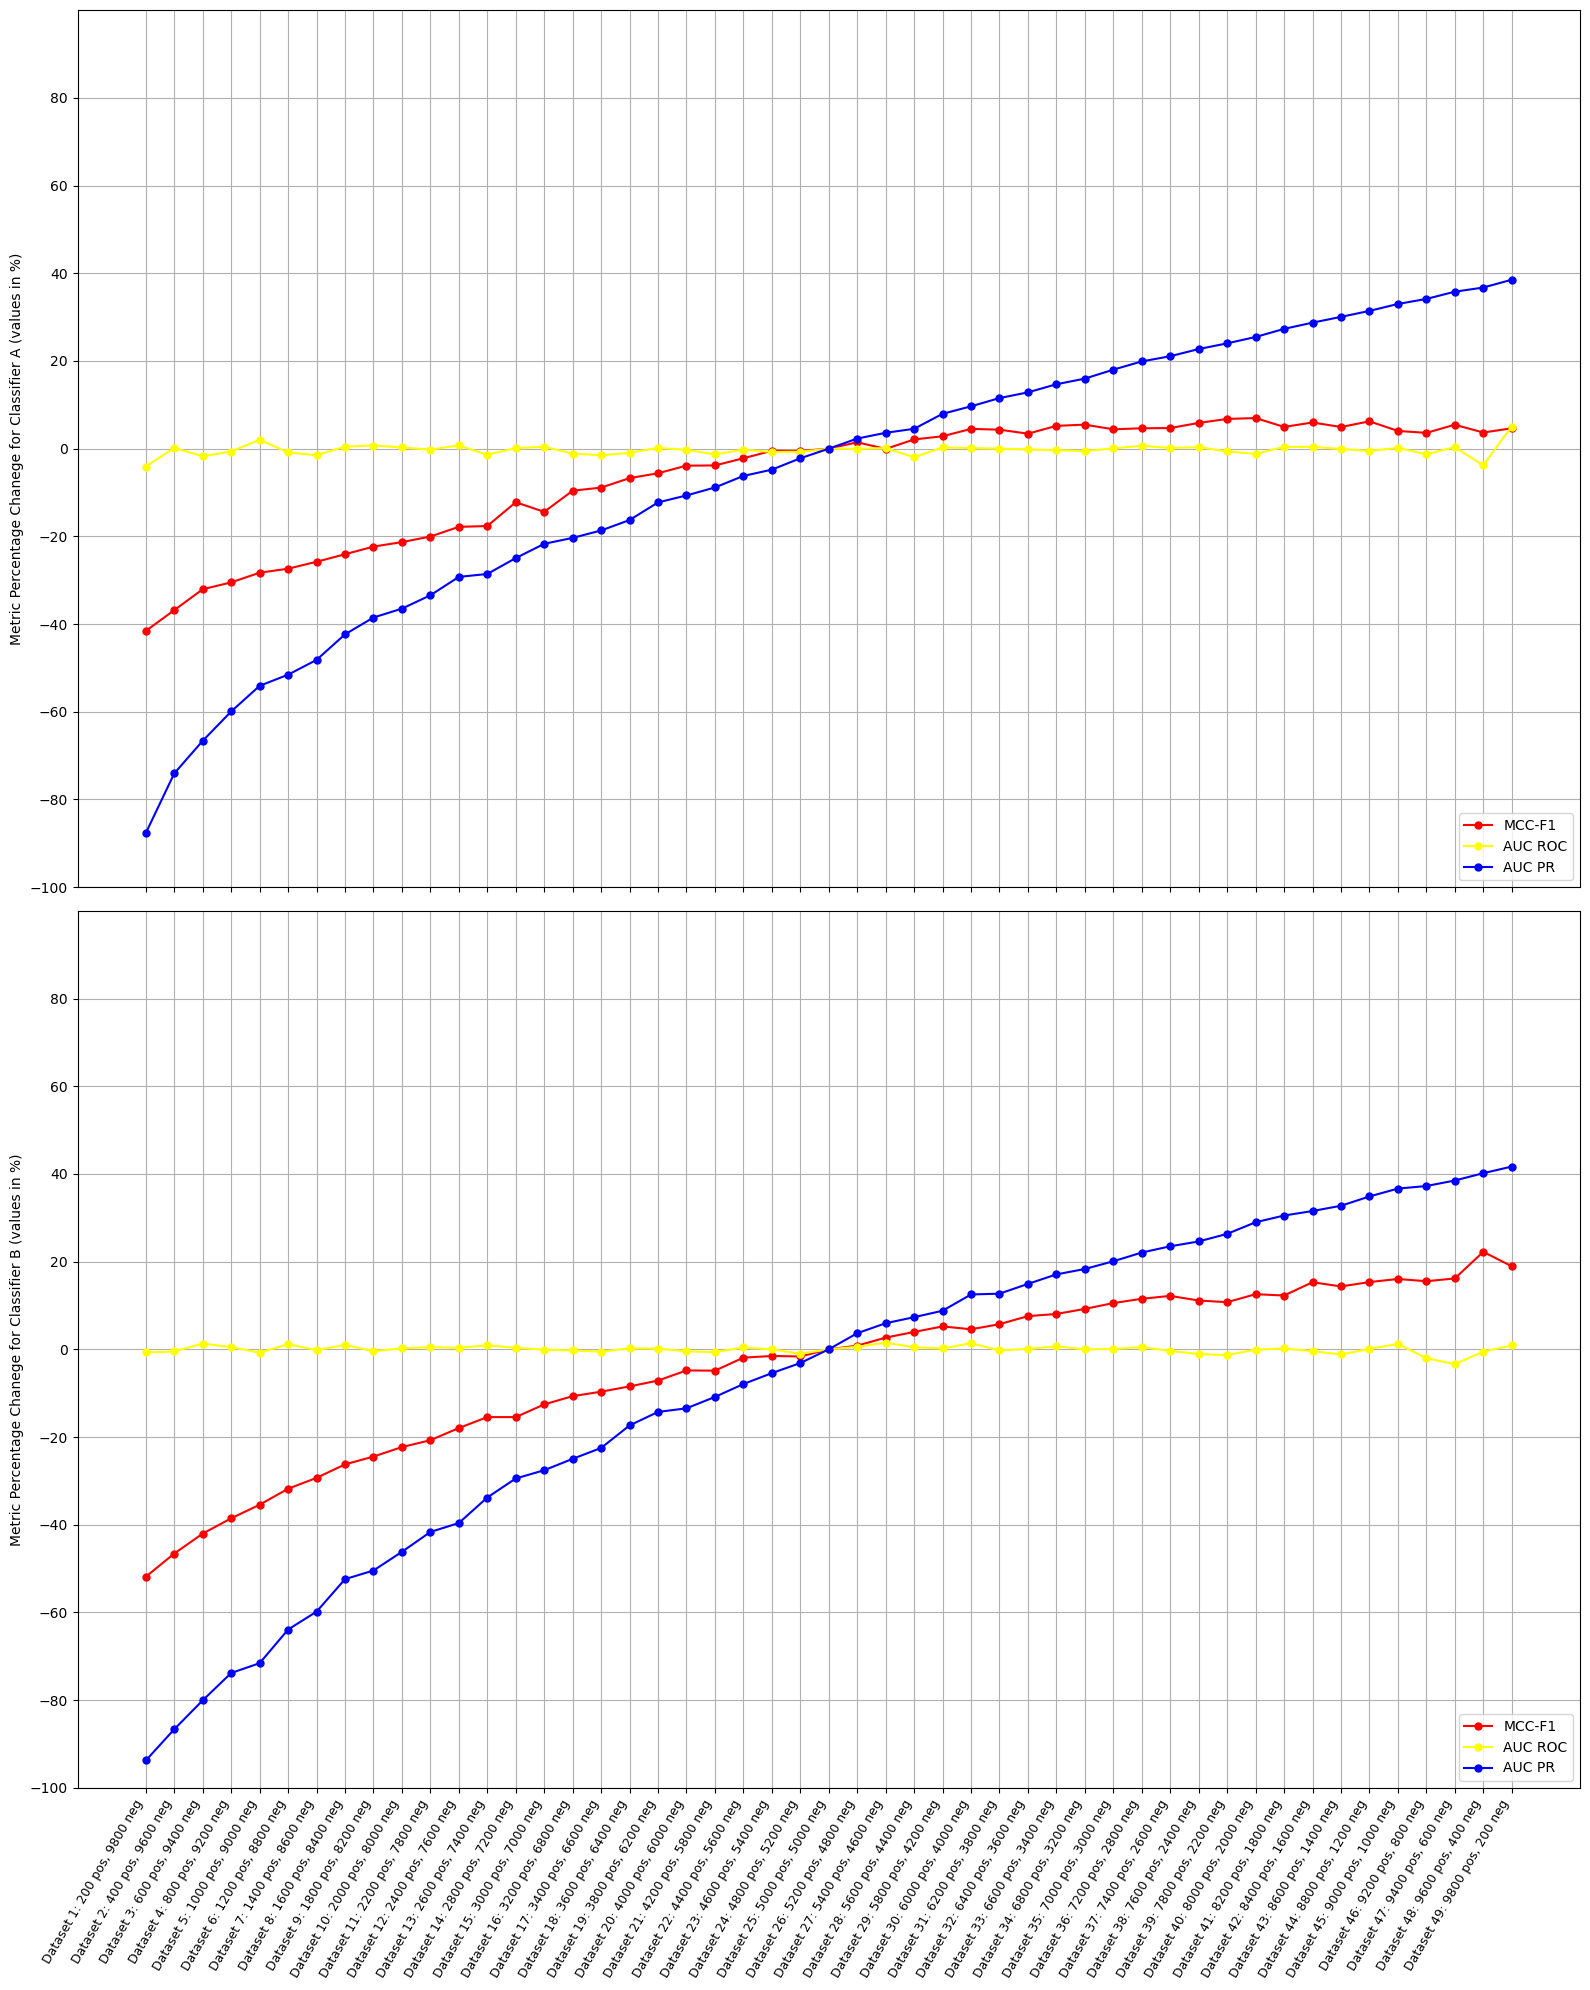
\includegraphics[scale=0.27]{Report/Figure/simulation2.jpg}
    \caption{Performance Percentage Change: the top plot shows the percentage change of 3 metrics for classifier A compared to the perfectly balanced dataset and similarly for classifier B at the bottom plot. The percentage change values at 7th dataset (in the middle) for all metrics and classifiers should always be 0.}
    \label{simulation2}
\end{figure}
\FloatBarrier

To investigate further, we conduct experiment 3. In this set up, we don't use any specific classifier but simply plot the different metrics as each element in the confusion matrix (\textit{TP}, \textit{TN}, \textit{FP}, \textit{FN}) varies. In each plot, we hold three elements constant and vary one. We create four plots in total, allowing us to examine whether certain metrics are sensitive to changes in confusion matrix elements. The datasets are not kept at a consistent size to allow for imbalanced scenarios. The results are shown in Figure \ref{simulation3}. In this experiment, we break down the \textbf{MCC-F1}, \textbf{ROC}, and \textbf{PR} metrics by plotting \textbf{MCC}, \textbf{F1 score}, \textbf{precision}, \textbf{recall}, and \textbf{FPR} separately. The definitions are given below: 
\[
\text{Precision} = \frac{TP}{TP + FP}, 
\text{Recall} = \frac{TP}{TP + FN}
\]
\[
\text{FPR} = \frac{FP}{FP + TN}, 
\text{F1} = 2 \times \frac{\text{Precision} \times \text{Recall}}{\text{Precision} + \text{Recall}}
\]
\[
\text{MCC} = \frac{(TP \times TN) - (FP \times FN)}{\sqrt{(TP + FP)(TP + FN)(TN + FP)(TN + FN)}}
\]
\\


\begin{figure}[hbt!]
    \centering
    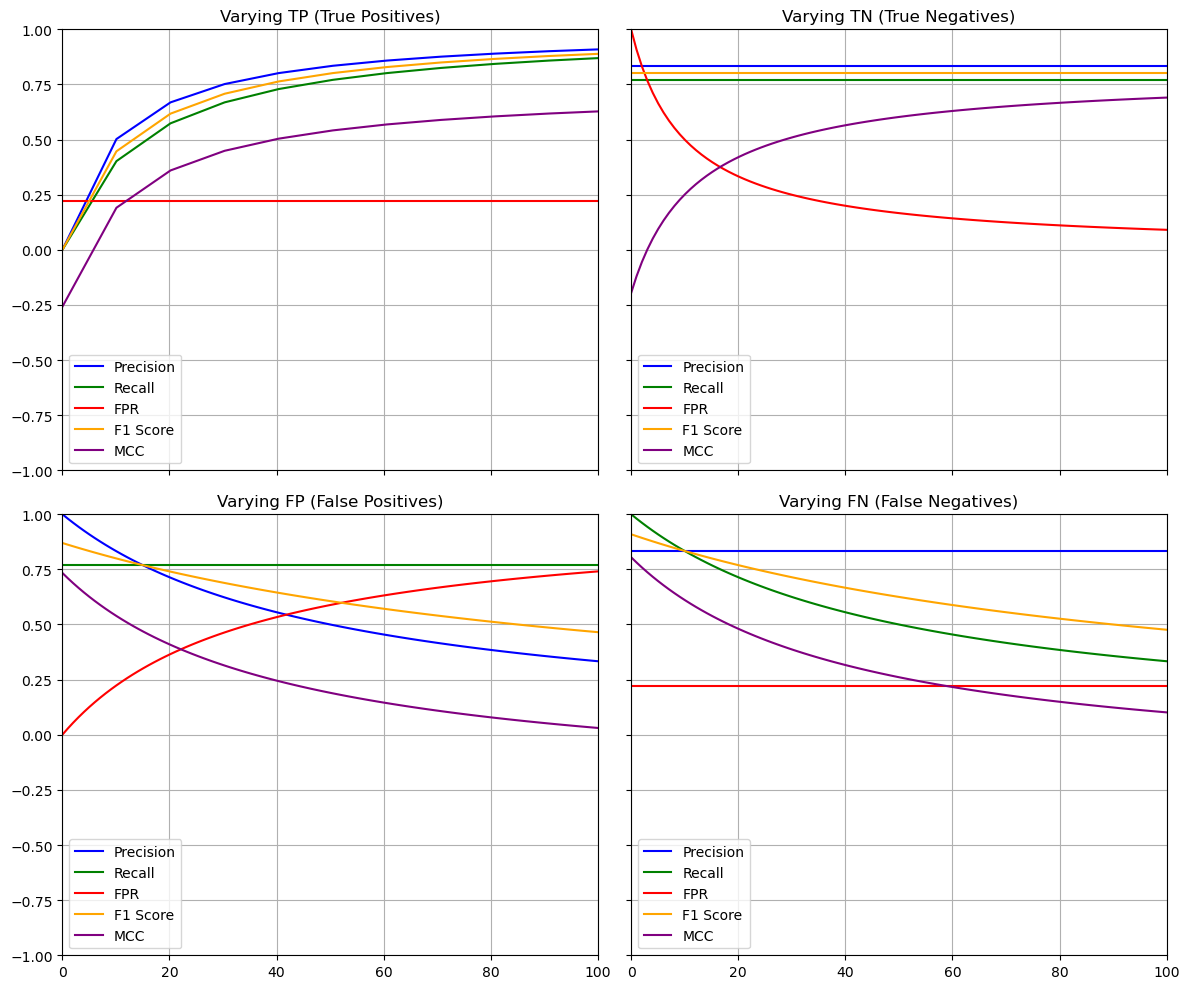
\includegraphics[scale=0.33]{Report/Figure/simulation3.jpg}
    \caption{}
    \label{simulation3}
\end{figure}
\FloatBarrier

As the results indicate, \textbf{FPR} is not sensitive to changes in \textit{TP} and \textit{FN}, while \textbf{precision}, \textbf{recall}, and \textbf{F1 score} are not sensitive to changes in \textit{TN}. Additionally, \textbf{recall} is not sensitive to changes in \textit{FP}, and \textbf{precision} and \textbf{FPR} are not sensitive to changes in \textit{FN}. These findings can also be inferred from the formulas that compose these metrics.\\

Due to the structure of the \textbf{ROC} curve, which plots \textbf{recall} against \textbf{FPR}, it makes sense why \textbf{ROC} does not perform well with negatively skewed datasets. In imbalanced datasets, especially when \textit{TN} greatly outnumbers \textit{TP}, even a rise in \textit{FP} may not significantly affect \textbf{FPR} due to the large number of negatives. Moreover, the classifier may increase \textit{TP} by lowering the threshold. This also increases \textit{FP}, but can be offset by the large number of \textit{TN}. If the classifier correctly identifies most positives, the \textbf{recall} may appear high, which can be misleading when combined with the low \textbf{FPR}. \\

In contrast, the \textbf{PR} curve performs better in negatively skewed datasets because it emphasizes the classifier's ability to predict the positive (minority) class. However, the \textbf{PR} curve loses its effectiveness in positively imbalanced datasets. With few negative instances, \textit{FP} has less impact on precision, and \textit{FN} has less impact on recall. Even if a classifier makes several \textit{FP}s, precision will not drop significantly because the total number of positives is large. Similarly, recall remains high as the number of \textit{FN} is small. Consequently, the \textbf{PR} curve becomes less informative in distinguishing between classifiers. \\

The \textbf{F1 score} faces similar advantages and challenges in both negatively and positively imbalanced datasets since it focuses on the positive class. However, \textbf{MCC} is sensitive to mis-classifications in both classes. It only achieves a high value when both \textit{TP} and \textit{TN} are high, and \textit{FP} and \textit{FN} are low. Therefore it provides a more comprehensive assessment for classifier performance across both the majority and minority classes. Overall, \textbf{MCC-F1} analysis offers more meaningful insights than \textbf{ROC} or \textbf{PR} analysis.  \\

It’s important to note that the choice of metrics is often depended on the specific task and its purpose. The \textbf{F1 score} (with $\beta=1$) finds a balance between Precision and Recall, making it useful when both false positives and false negatives are equally important in the analysis task. However, changing the $\beta$ value in the F-score can shift that balance. A higher $\beta$ (like \textbf{F2}) would place more weight on the Recall, which is ideal when missing positives is more costly. On the other hand, a lower $\beta$ (such as \textbf{F0.5}) would place more weight on the Precision, which is helpful when avoiding false positives is more critical. One can incorporate different F-scores in the MCC-F1 analysis to bring out different strengths and weaknesses of classifiers according to the problem setting.


\subsection{Optimal classifier across datasets}
A summary table for the classifiers performances in the previous simulation experiment 1 is presented in Figure \ref{simulation1_table}. Although in simulation 1, \textbf{classifier B} appears to perform better almost always than \textbf{classifier A}, we still observe cases when \textbf{classifier A} performs better than \textbf{classifier B}. This happens on the extremely negatively imbalanced datasets. Notice that how we constructed \textbf{classifier B} has an intuitive advantage over \textbf{classifier A} since we make a bigger difference in the positive class prediction scores for \textbf{classifier B}. Even under this "unfair" construction of the classifiers, we still cannot state that \textbf{classifier B} performs ultimately better under all circumstances. If we were to use the two classifiers on a target dataset that is extremely negatively imbalanced, say the ratio between positives and negatives is 1:100. As observing the current trend in the simulation, we cannot conclude that \textbf{classifier B} will perform better in this case. 

\begin{figure}[hbt!]
    \centering
    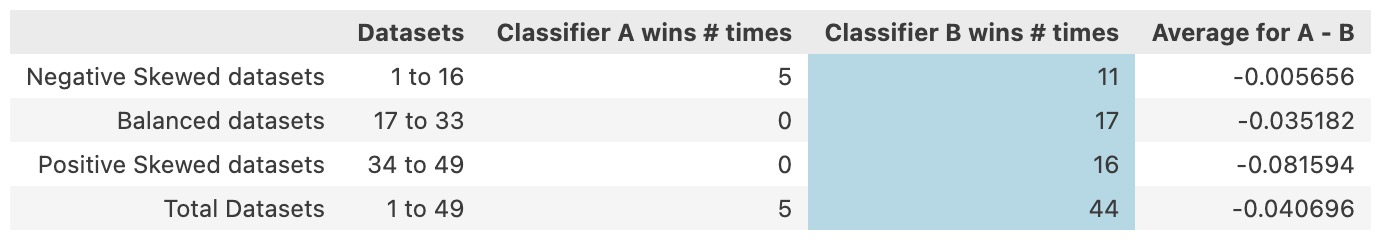
\includegraphics[scale=0.3]{Report/Figure/simulation1_table.jpg}
    \caption{Performance comparison between classifier A and classifier B: the winner for different types of datasets is highlighted in blue}
    \label{simulation1_table}
\end{figure}
\FloatBarrier

To elaborate on a more general context, we conduct experiment 4. In this simulation, we evaluate the performance of various machine learning classifiers across datasets with different levels of imbalance using the \textbf{MCC-F1} metric. We use five classifiers: \textbf{Logistic Regression}, \textbf{Support Vector Machine (SVM)}, \textbf{K-Nearest Neighbors (KNN)}, and \textbf{Naive Bayes}. For each classifier, we test its performance on 3 datasets: a balanced dataset (50\% positive, 50\% negative), a negatively imbalanced dataset (99\% negative, 1\% positive), and a positively imbalanced dataset (1\% negative, 99\% positive). Each dataset is generated using the \textit{make\_classification} function in the Python \textit{SKLearn} package. We control the datasets to be with 10,000 samples and 20 features. Each dataset is split into training and testing sets (with 30\% of data). After trained on the training set, each classifier outputs the prediction scores for the testing set. We then compute the \textbf{MCC-F1} metric on the testing set for evaluating the classifier's performance.\\

Finally, the results for all different classifiers and datasets are plotted in Figure \ref{simulation4}, where the \textbf{MCC-F1} metric value is plotted against the proportion of the number of negatives in the dataset. Comparing the classifier's performances across datasets, we see different classifier "winners". For the negatively imbalanced dataset, the \textbf{Logistic Regression} classifier outperforms other classifiers only slightly, with \textbf{Naive Bayes} classifier almost performs as good. For the balanced dataset, the \textbf{KNN} classifier outperforms other classifiers distinctively. And for the positively imbalanced dataset, the \textbf{Logistic Regression} classifier outperforms other classifiers moderately. This simulation demonstrates that the balance between positive and negative classes greatly influences the result of selecting a best classifier. There is no classifier that can universally outperforms others across different types of datasets. This is because that performance indeed depends on the class balance of the dataset and the evaluation metrics being used. A classifiers could obtain a very high performance score on imbalanced datasets, even if they simply predicts the majority class and ignores the minority class. 
\begin{figure}[hbt!]
    \centering
    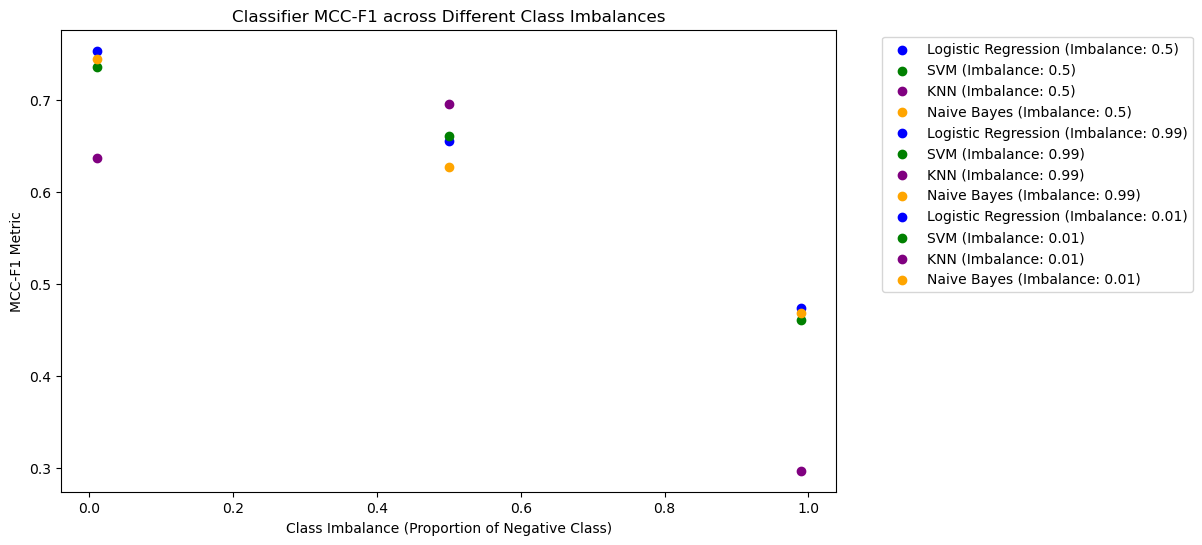
\includegraphics[scale=0.4]{Report/Figure/simulation4.jpg}
    \caption{}
    \label{simulation4}
\end{figure}
\FloatBarrier

\subsection{Summary}
In this extensional study, we explore beyond the original paper for the effectiveness of the MCC-F1 metric in contrast to other metrics (ROC and PR). Through a variety of experiment simulations, we highlight MCC-F1's advantage in imbalanced classification problems. However, the most suitable metric always depends on the specific goal of the task. We extend our exploration to the discussion point on whether the balance between positive and negative classes affects the choice for optimal classifier. In other words, we want to know if there is a single classifier that can consistently outperform others, regardless of the class distribution. Based on our findings, the answer is no. Since class balance does influence the classifier's performance substantially, there is no single classifier that can universally outperform across all datasets. 

\clearpage
\printbibliography
\end{document}
